\documentclass[11pt,a4paper]{article}
\usepackage[T1]{fontenc}
\usepackage[utf8]{inputenc}
\usepackage{lmodern}
\usepackage{amsmath,amssymb,amsthm,mathtools,mathrsfs}
\usepackage{graphicx,float,xcolor,multicol}
\usepackage[shortlabels]{enumitem}
\usepackage[margin=27mm]{geometry}
\usepackage{microtype,needspace,placeins}
\usepackage{tikz,tikz-cd}
\usetikzlibrary{arrows.meta,calc,positioning,patterns,decorations.pathreplacing}
\usepackage[colorlinks=true,linkcolor=teal,urlcolor=teal,citecolor=teal]{hyperref}
\setlength{\parindent}{0pt}
\setlength{\parskip}{.6em}
\setcounter{secnumdepth}{0}
\allowdisplaybreaks
\raggedbottom
\providecommand{\cross}{\times}
\DeclareUnicodeCharacter{2020}{\ensuremath{\dagger}}
\DeclareMathOperator{\supp}{supp}
\DeclareMathOperator*{\esssup}{ess\,sup}
\providecommand{\chapter}{\section}
\newenvironment{tool}[2]{\subsection*{Tool #1 --- #2}}{}
\newcommand{\ToolRef}[1]{Tool #1}
\newcommand{\FigureTag}[2]{\textit{Figure #1}}
\newcommand{\Result}[1]{\subsection*{#1}}
\newcommand{\Application}[1]{\subsubsection*{Application\if\relax\detokenize{#1}\relax\else\space--- #1\fi}}
\newcommand{\ProofHeading}{\par\textit{Proof.}\space}
\newcommand{\ProofOf}[1]{\par\textit{Proof of #1.}\space}
\newcommand{\RemarkHeading}{\par\textbf{Remark.}\space}
\newcommand{\NoteHeading}{\par\textbf{Note.}\space}
\newcommand{\ExerciseHeading}{\par\textbf{Exercise.}\space}

\graphicspath{{figures/elliptic-curves/}}
\begin{document}
\section*{Elliptic Curves — Algebraic Perspective}
% BLOG-CONTENT-BEGIN
\textbf{II) \underline{Algebraic Perspective}}

A smooth plane cubic curve is the following set:
$$C = \big\{[x:y:z]\in \mathbb{CP}^2  \big|   F(x, y, z) = 0,   \deg(F) = 3,   F\text{ is homogeneous}\big\},$$
where $\nabla F$ does not vanish at any point of $C$.
Let $P\in C$ be one of the nine points of inflection, and let $Q$ be a point on the tangent to $C$ at $P$. After choosing representatives of $P$ and $Q$ in $\mathbb{C}^3\backslash\{(0,0,0)\}$, a projective change of coordinates sends them to $(0,1,0)$ and $(1,0,0)$. Let the polynomial be
$$F(x,y,z) = \sum_{\substack{i,j\geq0\\i+j\leq3}}a_{ij}x^iy^jz^{3-i-j}$$
$[0:1:0] \in C$ implies $x=0$ is a root of the polynomial,
$$a_{30}x^3 + a_{21}x^2y+ a_{12}xy^2 + a_{03}y^3$$
By the way things have been set up, the line $[t:1:0]$ is tangent at $[0:1:0]$. Since $[0:1:0]$ is an inflection point, $x=0$ has multiplicity $3$ in the polynomial above. Hence $a_{21}=a_{12}=a_{03}=0$ and $a_{30}\neq0$. Let's now look at $F$ in the affine coordinate $z\neq 0$,
$$F(x,y,1) = y^2 -2(ax+b)y - P_3(x)$$

where the terms on the right-hand side have been extracted from the monomials $yz^2, xyz, z^2y$, and $x^3$, in that order. Complete the square by sending $y \rightarrow y-ax-b$ to obtain
$$y^2 = P_3(x) = (x-a)(x-b)(x-c)$$

This is the zero locus of $F$ in the transformed affine chart. Note that for the curve to be smooth $a, b, c$ must be distinct. Make a further change of coordinates by setting $X=(x-a)/(b-a)$, $Y=y/(b-a)^{3/2}$, and $\lambda=(c-a)/(b-a)$ to get,
$$Y^2 = X(X-1)(X-\lambda)$$

which with the transformation $X \rightarrow X + (1+\lambda)/3$ becomes,
$$Y^2 = X^3 + AX + B$$

The above is called the \textbf{Weierstrass normal form} of the cubic curve, which when graphed would look like:

\begin{figure}[htp]
            \centering
            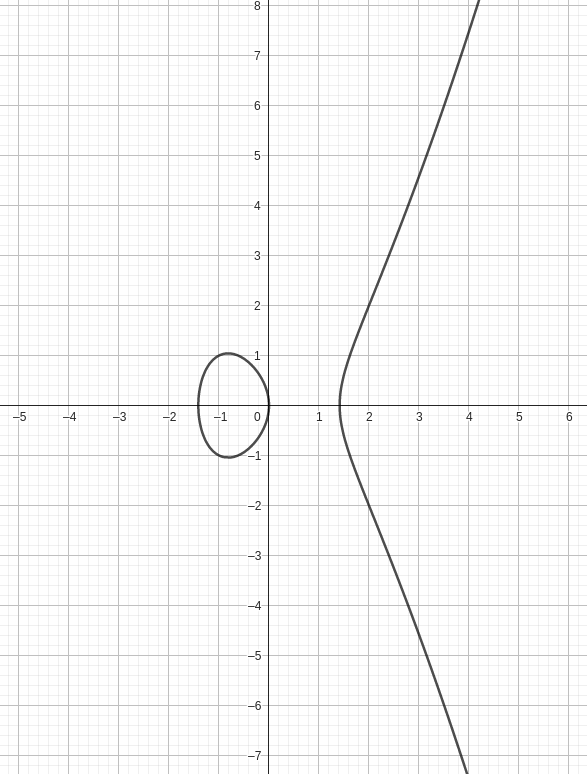
\includegraphics[width=0.58\linewidth]{Elliptic Curve.png}
        \end{figure}


In the geometric perspective, lattices appeared naturally as groups of symmetries. We shall now incorporate lattices to illuminate the algebraic perspective. Let $\Lambda = \mathbb{Z}\omega_1\oplus \mathbb{Z}\omega_2$ with $\text{Im}(\omega_1/\omega_2) >0$ (after scaling by $1/\omega_2$, it is equivalent to a lattice of the form $\mathbb{Z}\oplus\mathbb{Z}\tau$). Define,
$$\wp_{\Lambda} : \mathbb{C} \rightarrow \mathbb{CP}^1$$


$$\wp_{\Lambda}(z) := \frac{1}{z^2} + \sum_{\omega \in \Lambda\backslash \{0\}}\bigg(\frac{1}{(z-\omega)^2} - \frac{1}{\omega^2}\bigg)$$

The object defined above goes by the name \textbf{Weierstrass $\wp$ function}. Let us study its nature to reveal the cameo of lattices for cubic curves; we shall do it in four steps.

\subsection*{Convergence} Note that,
$$\bigg|\frac{1}{(z-\omega)^2} - \frac{1}{\omega^2}\bigg| = \bigg|\frac{2z\omega - z^2}{\omega^2(z-\omega)^2}\bigg| = \bigg|\frac{\omega}{\omega^4}\bigg(\frac{2z-z^2\omega^{-1}}{(z\omega^{-1} - 1)^2}\bigg)\bigg| =: \frac{A(z,\omega)}{|\omega|^3}$$

If $K\subset\mathbb C\setminus\Lambda$ is compact and $z\in K$, then dist$(K, \Lambda) > \epsilon$, as a result $z\omega^{-1} - 1$ is bounded away from $0$ for $|\omega|$ large enough. For $|\omega|$ large enough note that $A(z, \omega) \to 2|z|$, and as $z\in K$, we see that $A(z, \omega)$ is uniformly bounded on $K$. Hence,

$$\bigg|\frac{1}{(z-\omega)^2} - \frac{1}{\omega^2}\bigg| = \mathcal{O}\bigg(\frac{1}{|\omega|^3}\bigg)$$

Now,

$$\sum_{\omega \in \Lambda\backslash \{0\}} \frac{1}{|\omega|^3} = \sum_{n=1}^{\infty}\Bigg(\sum_{\text{max}(|p|, |q|) = n} |p\omega_1 + q\omega_2|^{-3}\Bigg) \leq \sum_{n = 1}^{\infty}\frac{8n}{(nh)^3}$$


where $h$ is the smaller of the heights of the parallelogram generated by $0$, $\omega_1$, $\omega_2$, and $\omega_1+\omega_2$ (called the \textbf{fundamental parallelogram} of $\Lambda$). The last inequality above is illustrated below.

\begin{figure}[htp]
            \centering
            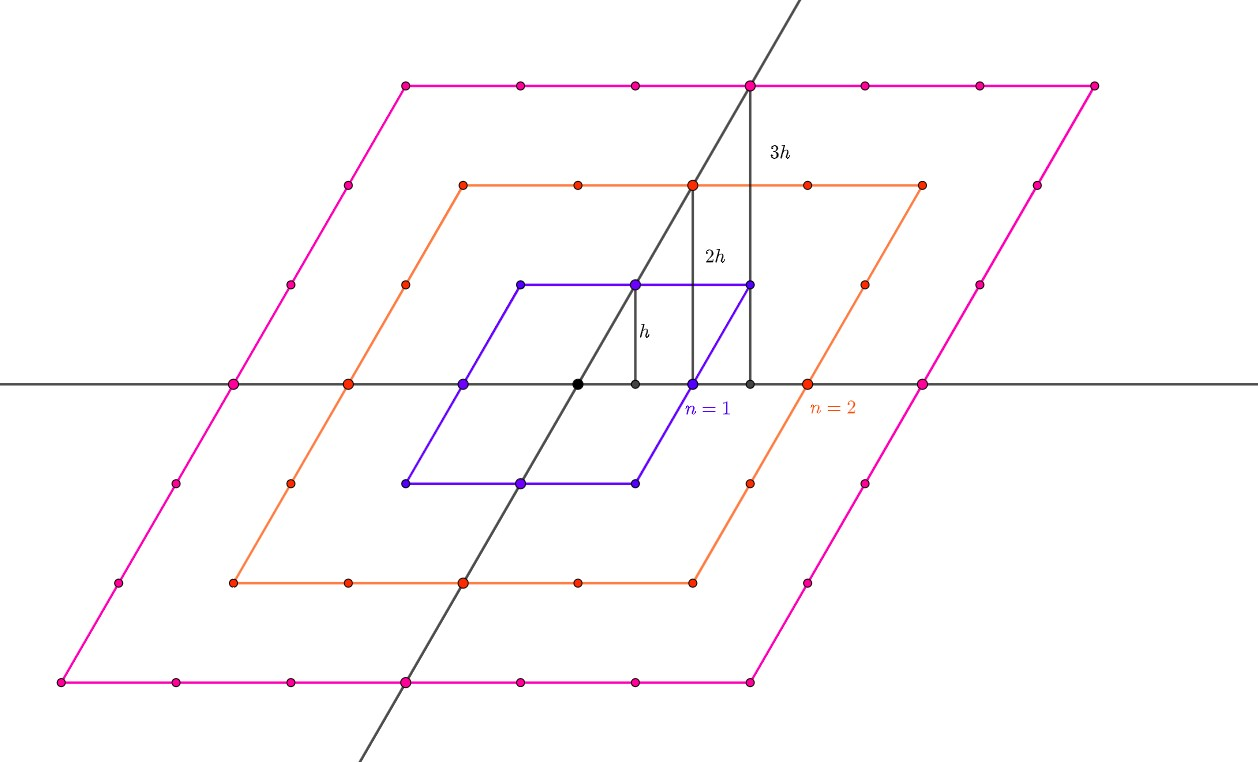
\includegraphics[width=0.96\linewidth]{Inequality.jpg}
        \end{figure}


Since a uniform limit of holomorphic functions is holomorphic, we have $\wp_{\Lambda}(z) \in \mathcal{O}(\mathbb{C}\backslash\Lambda)$ with poles of order $2$ on $\Lambda$.

\subsection*{Periodicity} Clearly,
$$\wp_{\Lambda}'(z) = -\frac{2}{z^3}-2\sum_{\omega\in\Lambda\setminus\{0\}}\frac{1}{(z-\omega)^3}$$

has periods $\omega_1$ and $\omega_2$. The same is true of
$$\wp_{\Lambda}(z) = \frac{1}{z^2} + \sum_{\omega \in \Lambda\backslash \{0\}}\bigg(\frac{1}{(z-\omega)^2} - \frac{1}{\omega^2}\bigg)$$

\subsection*{Zeros and poles} Note that The doubly periodic functions $\wp_{\Lambda}$ and $\wp_{\Lambda}'$ descend to ramified covers $\mathbb{C}/\Lambda\to\mathbb{CP}^1$ of degrees $2$ and $3$, respectively. Now as $\wp_{\Lambda}'(z)$ is odd we get,

$$\wp_{\Lambda}'(\omega_i/2) = -\wp_{\Lambda}'(-\omega_i/2) = -\wp_{\Lambda}'(\omega_i - \omega_i/2)$$
which implies,

$$\wp_{\Lambda}'\bigg(\frac{\omega_1+\omega_2}{2}\bigg) = \wp_{\Lambda}'\bigg(\frac{\omega_1}{2}\bigg) = \wp_{\Lambda}'\bigg(\frac{\omega_2}{2}\bigg) = 0$$

These are the only zeroes of $\wp_{\Lambda}'$ since it induces a $3$-fold ramified cover. Let,
$$e_1 = \wp_{\Lambda}\bigg(\frac{\omega_1}{2}\bigg),   e_2 = \wp_{\Lambda}\bigg(\frac{\omega_1+\omega_2}{2}\bigg),   \text{and }e_3 = \wp_{\Lambda}\bigg(\frac{\omega_2}{2}\bigg)$$

By Riemann-Hurwitz formula the three half-periods and $[\Lambda]$ are the only ramification points of the $2$-fold cover that $\wp_{\Lambda}$ induces, each with ramification index $2$; the corresponding branch values are $\{e_i\}_i$ and $\infty$, which forces the $e_i$ to be distinct.

\subsection*{Differential equation} Consider,

$$H(z) = \wp_{\Lambda}'(z)^2-4(\wp_{\Lambda}(z) - e_1)(\wp_{\Lambda}(z) - e_2)(\wp_{\Lambda}(z) - e_3)$$

Then $H$ is a doubly periodic entire function, meaning $H(z) = c$. At a half-period, both terms vanish, so $c=0$. Therefore,
$$\wp_{\Lambda}'(z)^2 = 4(\wp_{\Lambda}(z) - e_1)(\wp_{\Lambda}(z) - e_2)(\wp_{\Lambda}(z) - e_3)$$

With the help of basic properties of the Weierstrass function expounded above, we construct the following map:

$$\Phi : \mathbb{C} \rightarrow \mathbb{CP}^2$$


$$\Phi(z):= \begin{cases}
[\wp_{\Lambda}(z):\wp_{\Lambda}'(z):1], & \text{ if } z \notin \Lambda\\
[0:1:0], & \text{ else }
\end{cases}$$
Clearly, $\Phi$ factors through the complex torus to yield $\widetilde{\Phi}$,
\[\begin{tikzcd}[row sep=large,column sep=large,cells={nodes={font=\large}}]
	{\mathbb{C}} && {\mathbb{CP}^2} \\
	& {\mathbb{C}/\Lambda}
	\arrow["\Phi", from=1-1, to=1-3]
	\arrow["\pi"', from=1-1, to=2-2]
	\arrow["{\widetilde{\Phi}}"', from=2-2, to=1-3]
\end{tikzcd}\]

The map $\widetilde{\Phi}$ is clearly an analytic embedding whose image lies in the smooth cubic curve. Indeed, the map near $0$ is given by $$z \rightarrow \bigg[\frac{\wp_{\Lambda}(z)}{\wp_{\Lambda}'(z)}:1:\frac{1}{\wp_{\Lambda}'(z)}\bigg]$$

This proves analyticity at $0$. Moreover, the inverse image of $[0:1:0]$ in $\mathbb{C}/\Lambda$ is $[\Lambda]$, so the map is one-to-one and hence an embedding. Therefore, lattices parameterize smooth cubic curves.

\textbf{Remark.} We managed to show that all genus $1$ Riemann surfaces can be embedded into a smooth cubic curve. It is important to note that we haven't proved the equivalence of geometric and algebraic perspectives, for such a thing would amount to constructing a cubic curve whose zero locus is a given genus $1$ Riemann surface; we're merely capable of constructing one isomorphic to it.

% BLOG-CONTENT-END
\end{document}
